% ------------------------------------------------------------------------------
% LaTeX template created by
% Iker Algañaraz, May Juarez F., Gastón A. Lozano S., Belén N. Paz
% ------------------------------------------------------------------------------

\documentclass[a4paper,12pt]{article}

% ------------------------------------------------------------------------------
% Packages
% ------------------------------------------------------------------------------
\usepackage{anysize} % Márgenes
\usepackage[hypcap=false, font=small, justification=centering, labelfont=bf]{caption} % Pie de foto/tabla
\usepackage{multicol} % Columnas
\usepackage{amsmath} % Fórmulas matemáticas
\usepackage{amssymb} % Símbolos matemáticos
\usepackage{amsfonts} % Font matemática
\usepackage[utf8]{inputenc} % Facilitar la escritura en español
\usepackage{xcolor} % Color del texto
\usepackage{graphicx} % Figuras
\usepackage[spanish,es-tabla]{babel} % Tipografía del idioma
\usepackage{booktabs} % Separación en tablas
\usepackage{multirow} % Multirow en tablas
\usepackage{hyperref} % Refs como hyperlinks
%\usepackage{biblatex} % Bibliografía automática a partir de base bib

%\usepackage{array}
%\usepackage{verbatim}% Comentarios multilinea
%\usepackage{siunitx} % Unidades del sistema internacional
%\usepackage{fancyhdr} % Personalizar encabezado y pie de pagina
%\usepackage{longtable} % Tablas largas
%\usepackage{blindtext} % Lore ipsum
%\usepackage{soul} % Subrayar
%\usepackage{grffile}
%\usepackage{mathrsfs}

% ------------------------------------------------------------------------------
% Config
% ------------------------------------------------------------------------------
\newenvironment{Figure}
  {\par\medskip\noindent\minipage{\linewidth}}
  {\endminipage\par\medskip}

\providecommand{\abs}[1]{\lvert#1\rvert} % Valor absoluto

\marginsize{2cm}{2cm}{1cm}{2cm} % pkg: anysize

\graphicspath{{./Fotos/}} % pkg: graphicx

\setlength\columnsep{18pt}
\setlength\parskip{4pt} \setlength\parindent{0in}

\title{ Interferencia en películas delgadas \\ 
\medskip \large Universidad Nacional de Tucumán}
\author{May Juarez Ferriol}
\date{}

% ------------------------------------------------------------------------------
% Document
% ------------------------------------------------------------------------------
\begin{document}

\maketitle

\section*{Franjas de interferencia}

    \begin{Figure}
        \centering

        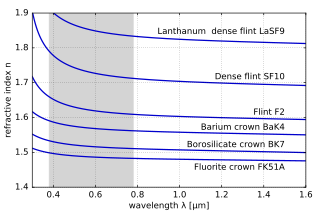
\includegraphics[width=0.5\linewidth]{flint.png}
        \captionof{figure}{Índice de refracción en función de longitud de onda para varios materiales}
        \label{fig: nLambda}
    \end{Figure}

    De la figura \ref{fig: nLambda}, obtenemos los valores:

    \begin{align*}
        &n = 1.775 \ para \ 400 \ nm\\
        &n = 1.725 \ para \ 600 \ nm
    \end{align*}

    Si la película tiene espesor t, la luz tiene incidencia normal y longitud de onda l en la película; si ninguna o si ambas ondas reflejadas en las dos superficies tienen un desplazamiento de fase de medio ciclo por reflexión, las condiciones para que haya interferencia constructiva son las dadas por la ecuación (\ref{eq: interferenciaConstructiva}). \cite{Sears}

    \begin{equation}
        2t=m \lambda \ \ \ \ (m=0, 1, 2, ...)
        \label{eq: interferenciaConstructiva}
    \end{equation}

    En nuestro caso, la longitud de onda estará dada por la ecuación (\ref{eq: lambda}). \cite{Sears}

    \begin{equation}
        \lambda = \frac{\lambda_0}{n}
        \label{eq: lambda}
    \end{equation}

    Por lo tanto, el grosor de la cuña en distintas posiciones será el mostrado en las tablas \ref{tab: flint} y .

    \begin{Figure}
        \centering

        \begin{tabular}{c|c}
            Índice de refracción & Longitud de onda [nm]\\
            1.775 & 225 \\
            \midrule
            N$^\circ$ de mínimo & Grosor de cuña [nm] \\
            0 & 0 \\
            1 & 112.5 \\
            2 & 225.0 \\
            3 & 337.5 \\
            4 & 450.0 \\
            5 & 562.5 \\
        \end{tabular}

        \label{tab: flint}
    \end{Figure}

    \begin{Figure}
        \centering

        \begin{tabular}{c|c}
            \toprule
            Índice de refracción & Longitud de onda [nm]\\
            1.725 & 348 \\
            \midrule
            N$^\circ$ de mínimo & Grosor de cuña [nm] \\
            0 & 0 \\
            1 & 174.0 \\
            2 & 348.0 \\
            3 & 522.0 \\
            4 & 696.0 \\
            5 & 870.0 \\
        \end{tabular}

        \captionof{table}{}
        \label{tab: flint2}
    \begin{Figure}

\begin{thebibliography}{99}

\bibitem{Sears} H. D. Young, R. A. Freedman. \emph{Sears and Zemansky's University Physics: with Modern Physics}, 14th ed. (Pearson, Boston, 2016), p. 1169, 1172.

\bibitem{} R. A. Serway, C. Vuille. \emph{College Physics}, 11th ed. (Cengage, Australia, 2018)

\bibitem{} R. A. Serway, J. W. Jewett. \emph{Physics for Scientists and Engineers with Modern Physics}, 10th ed. (Cengage, Australia, 2017)

\end{thebibliography}

\end{document}

% ------------------------------------------------------------------------------
% Common references and examples
% ------------------------------------------------------------------------------
% 
% ---------------------------
% Bibliography
% ---------------------------
% \bibitem{} Sears, Zemansky. \emph{Física universitaria}, vol. 2, 14th ed. Pearson Education, 2018.
% \bibitem{} Hecht, Zajac. \emph{Óptica}, 4th ed. Pearson Education, 2003.
% \bibitem{} Serway, Jewett. \emph{Physics for Scientists and Engineers}, vol. 2, 6th ed. Brooks Cole, 2004.
% \bibitem{} Jenkins, White. \emph{Fundamentos de óptica}, 3th ed. Aguilar S.A., 1964.
%
% ---------------------------
% Tables
% ---------------------------
% \begin{Figure}
%     \centering
%
%     \begin{tabular}{c|c}
%         \toprule
%          & \textit{...} \\
%          & \textit{[]} \\
%         \midrule
%         ... & \multirow{2}{*}{$(... \pm ...)$} \\
%         ... & \\
%         ... & \multirow{2}{*}{$(... \pm ...)$} \\
%         ... & \\ \hline
%         ... & $(... \pm ...)$ \\
%         ... & $(... \pm ...)$ \\
%         \bottomrule
%     \end{tabular}
%
%     \captionof{table}{}
%     \label{tab:}
% \end{Figure}
%
% \begin{Figure}
%     \centering
%
%     \begin{tabular}{cc}
%         \toprule
%         \textit{\textbf{... []}} & \textit{\textbf{$... []}}\\
%         \midrule
%         $... \pm ...$ & $... \pm ...$ \\
%         $... \pm ...$ & $... \pm ...$ \\
%         \bottomrule
%     \end{tabular}
%
%     \captionof{table}{}
%     \label{tab:}
% \end{Figure}
%
% ---------------------------
% Figures
% ---------------------------
% \begin{Figure}
%     \centering
%     \includegraphics[width=1\linewidth]{.jpg}
%     \captionof{figure}{}
%     \label{fig:}
% \end{Figure}
%
% ---------------------------
% Equations
% ---------------------------
% \begin{equation}
%     \label{eq:}
%     ...
% \end{equation}